\section{K-Nearest Neighbors (KNN) Model Visualizations}\label{annexe:knn_visualizations}

\subsubsection{KNN Model Performance Metrics}
Training performance is perfect across all metrics, indicating clear overfitting. Validation and test accuracy remain high; however, precision and F1-score are substantially lower due to class imbalance. Recall is moderate, while specificity remains high, showing strong performance on the majority class. MCC values indicate limited but non-random predictive capability on unseen data.

\begin{figure}[H]
    \centering
    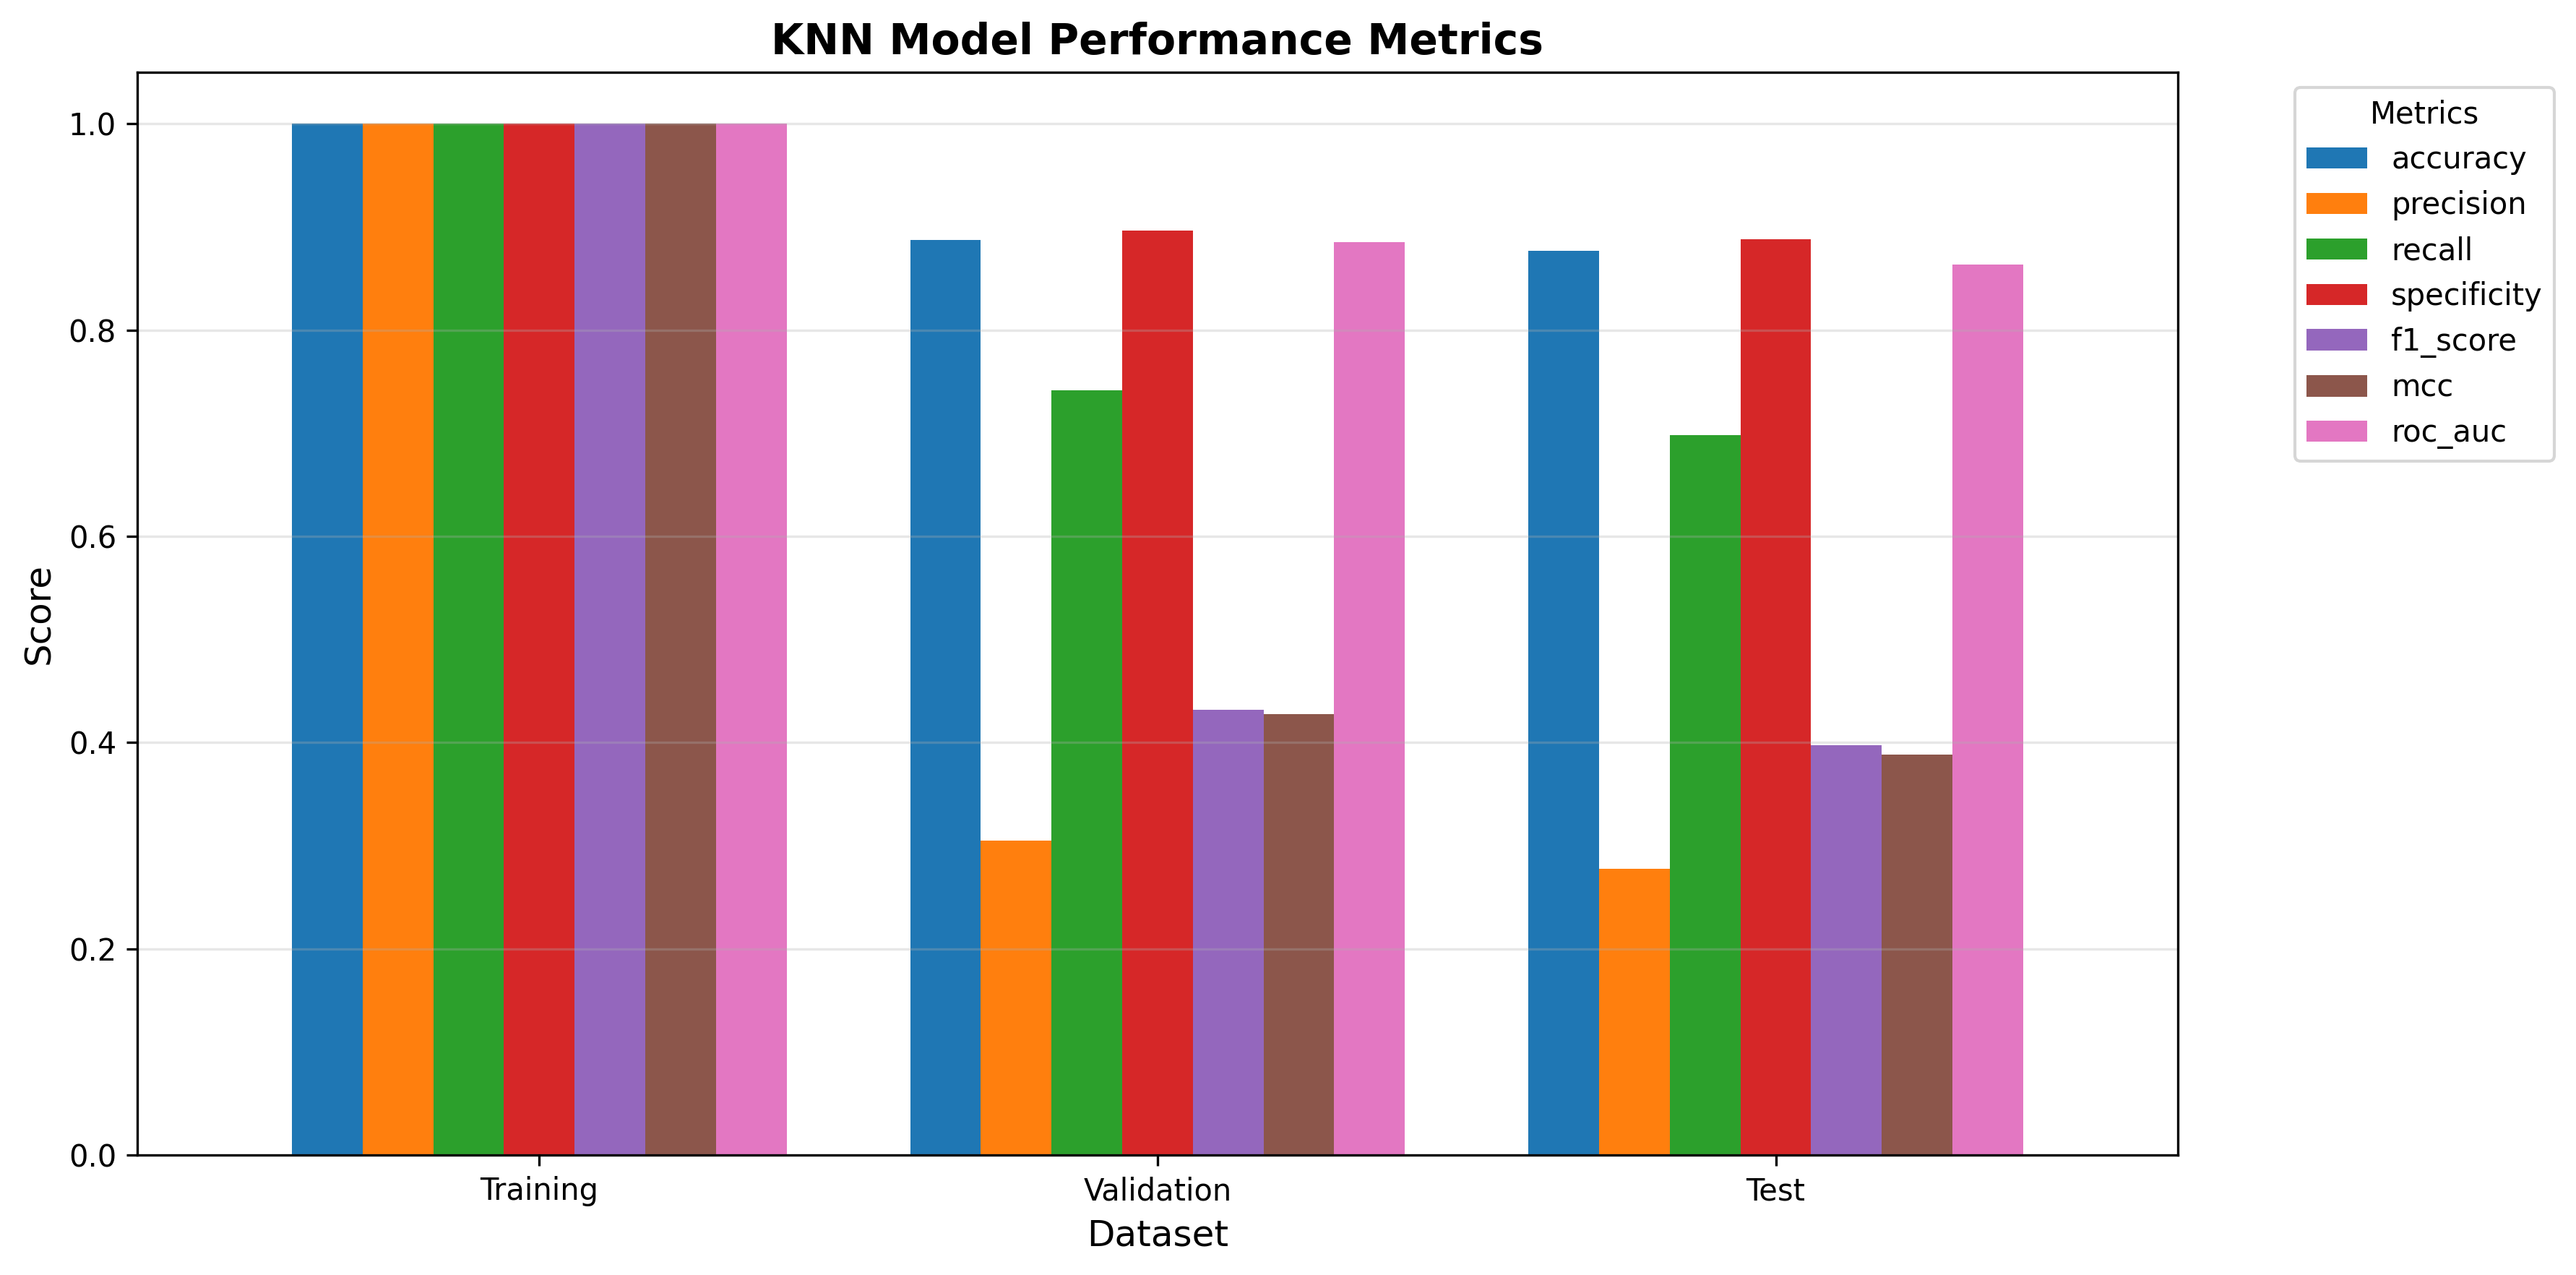
\includegraphics[width=0.5\linewidth]{images/KNN/metrics_comparison_KNN_predefined.png}
    \caption{Comparison of performance metrics for the predefined KNN model.}
    \label{fig:metrics_comparison_knn_predefined}
\end{figure}

\subsubsection{Confusion Matrices}
The training confusion matrix shows perfect classification with no errors. Validation and test matrices exhibit a limited number of false negatives and a higher number of false positives, leading to reduced precision but acceptable recall. Error patterns are consistent across validation and test sets.
\begin{figure}[H]
    \centering
    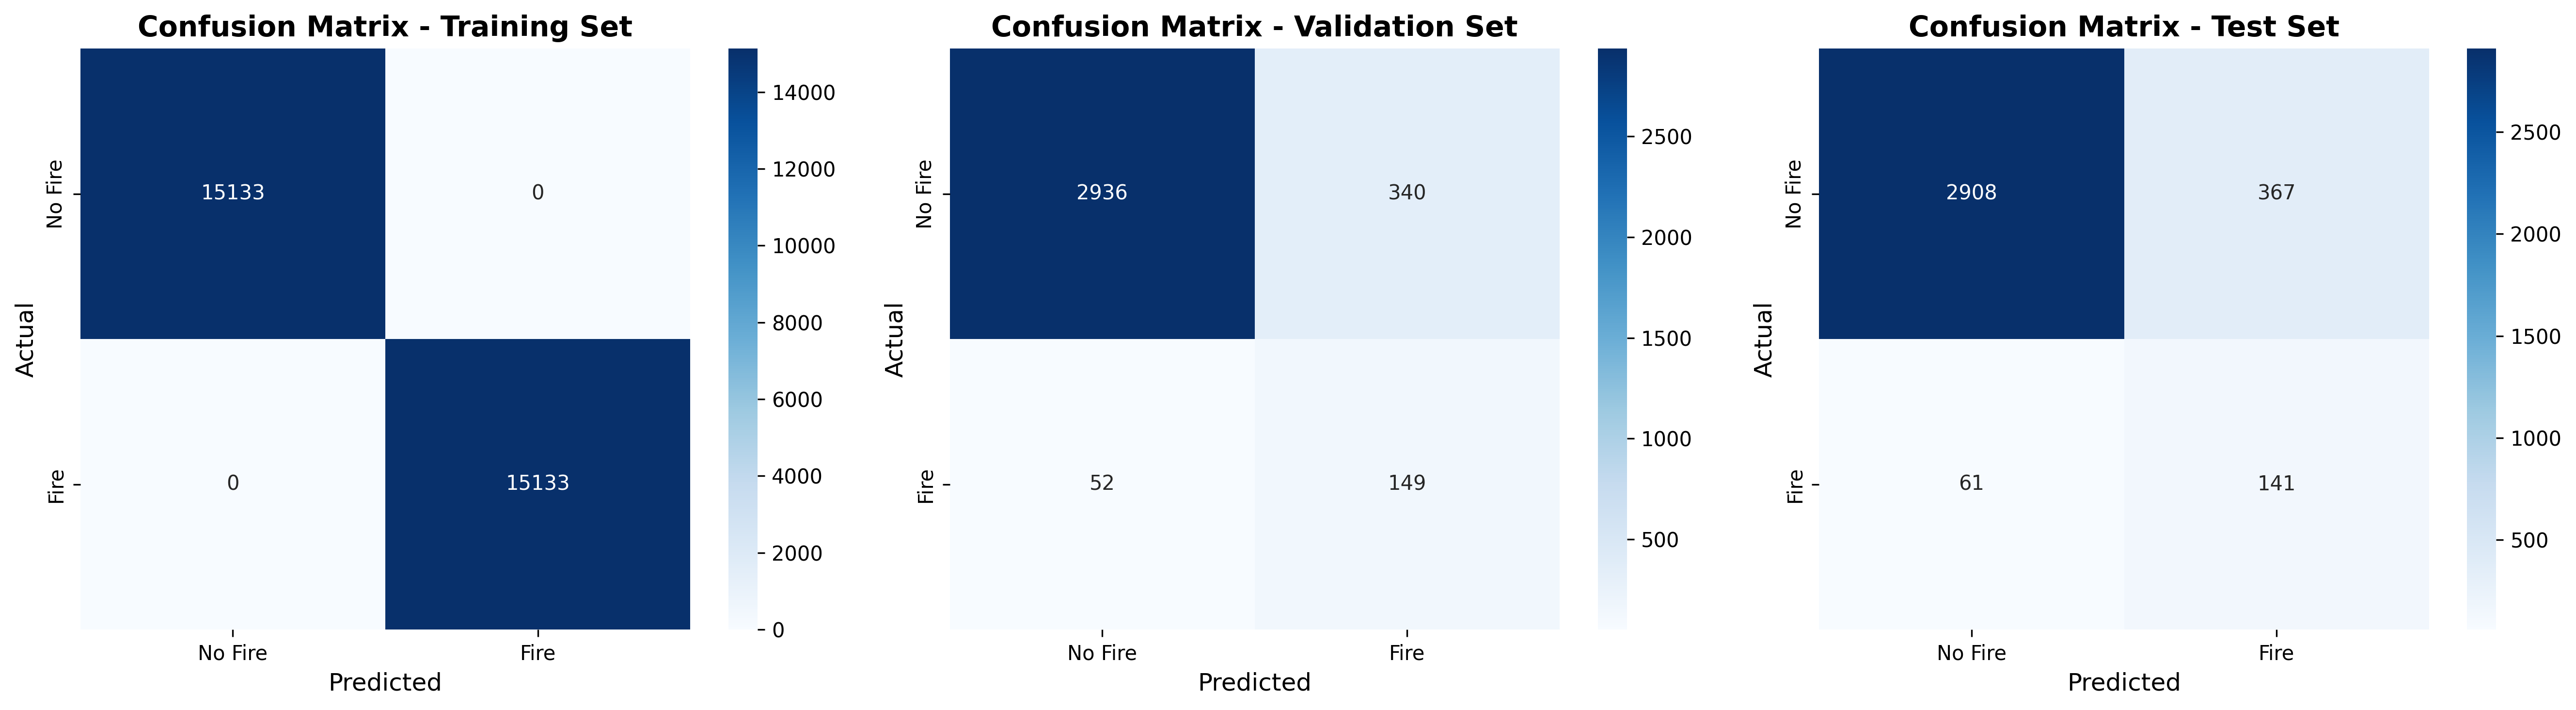
\includegraphics[width=0.5\linewidth]{images/KNN/confusion_matrices_KNN_predefined.png}
    \caption{Confusion matrices for the predefined KNN model.}
    \label{fig:confusion_matrices_knn_predefined}
\end{figure}

\subsubsection{ROC Curves}
The training ROC curve achieves an AUC of 1.00, confirming overfitting. Validation and test ROC curves achieve AUC values of approximately 0.89 and 0.86, respectively, indicating good discriminative performance. Both curves remain well above the random classifier baseline.

\begin{figure}[H]
    \centering
    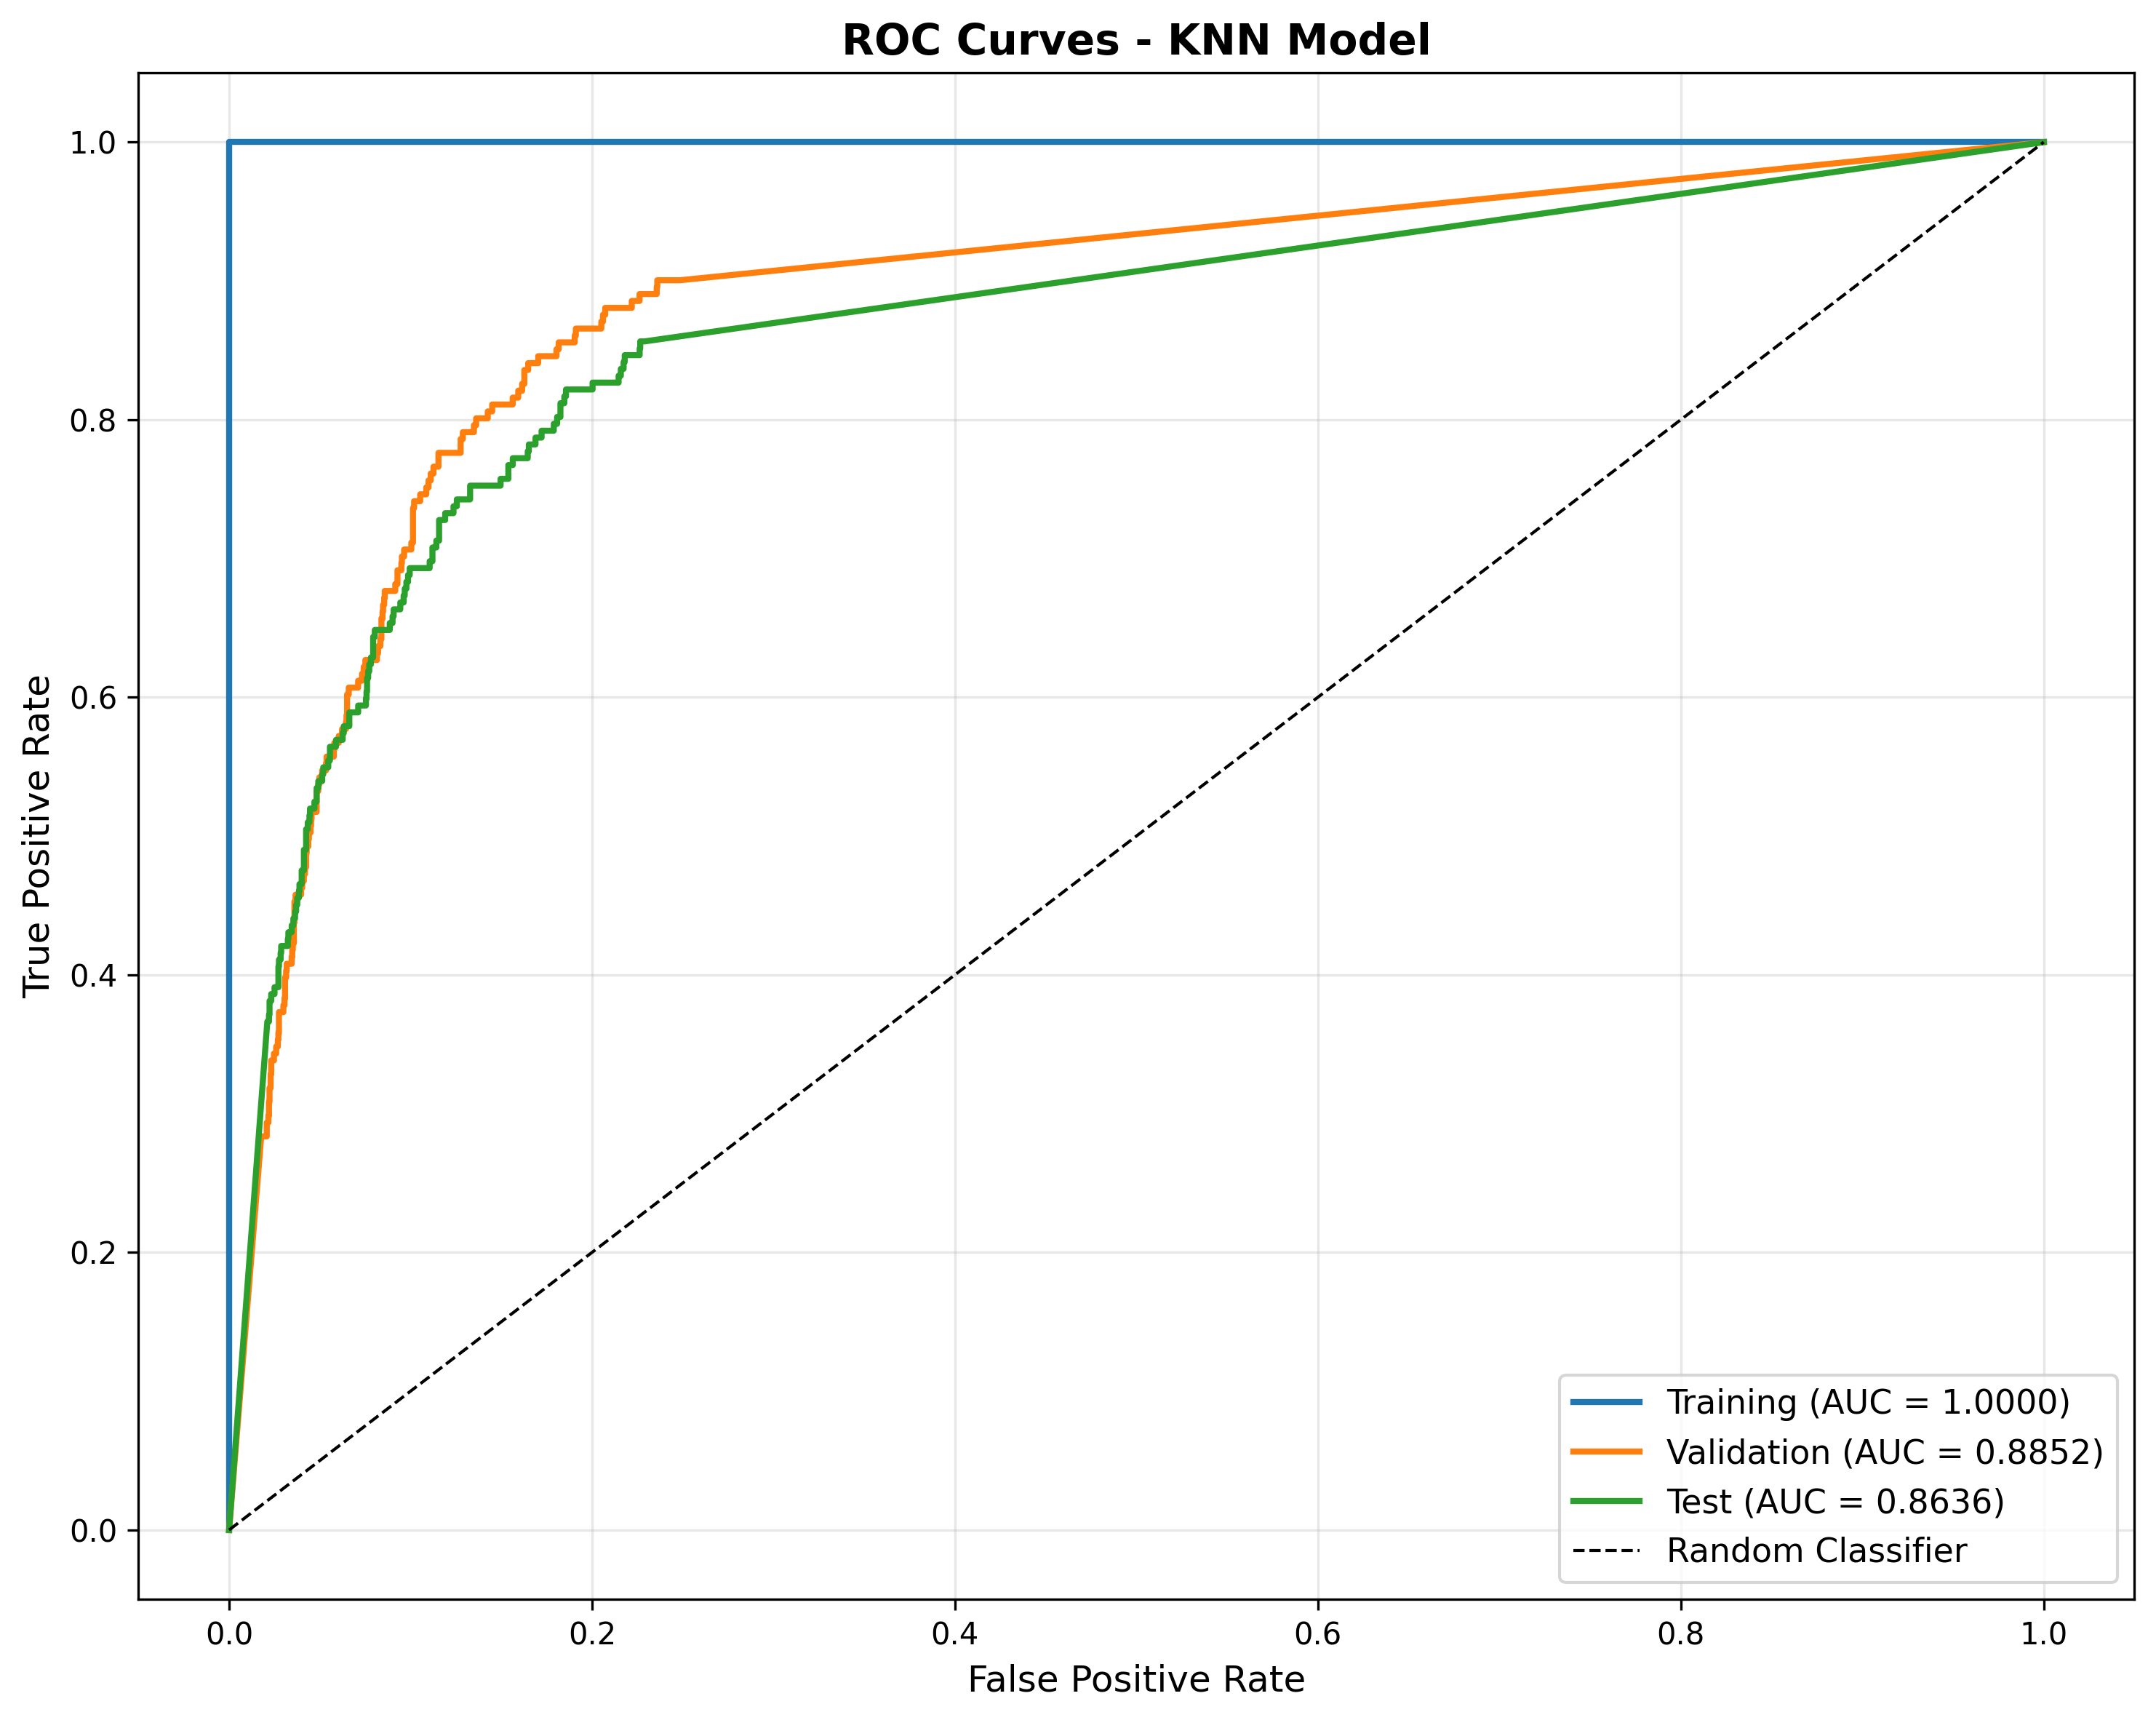
\includegraphics[width=0.5\linewidth]{images/KNN/roc_curves_KNN_predefined.png}
    \caption{ROC curves for the predefined KNN model.}
    \label{fig:roc_curves_knn_predefined}
\end{figure}

\subsubsection{Threshold Optimization Analysis}
Increasing the classification threshold results in decreasing recall and increasing precision and specificity. The F1-score and MCC reach their maximum values near the selected threshold of 0.50. False negatives increase with higher thresholds, highlighting the cost of conservative decision boundaries.
\begin{figure}[H]
    \centering
    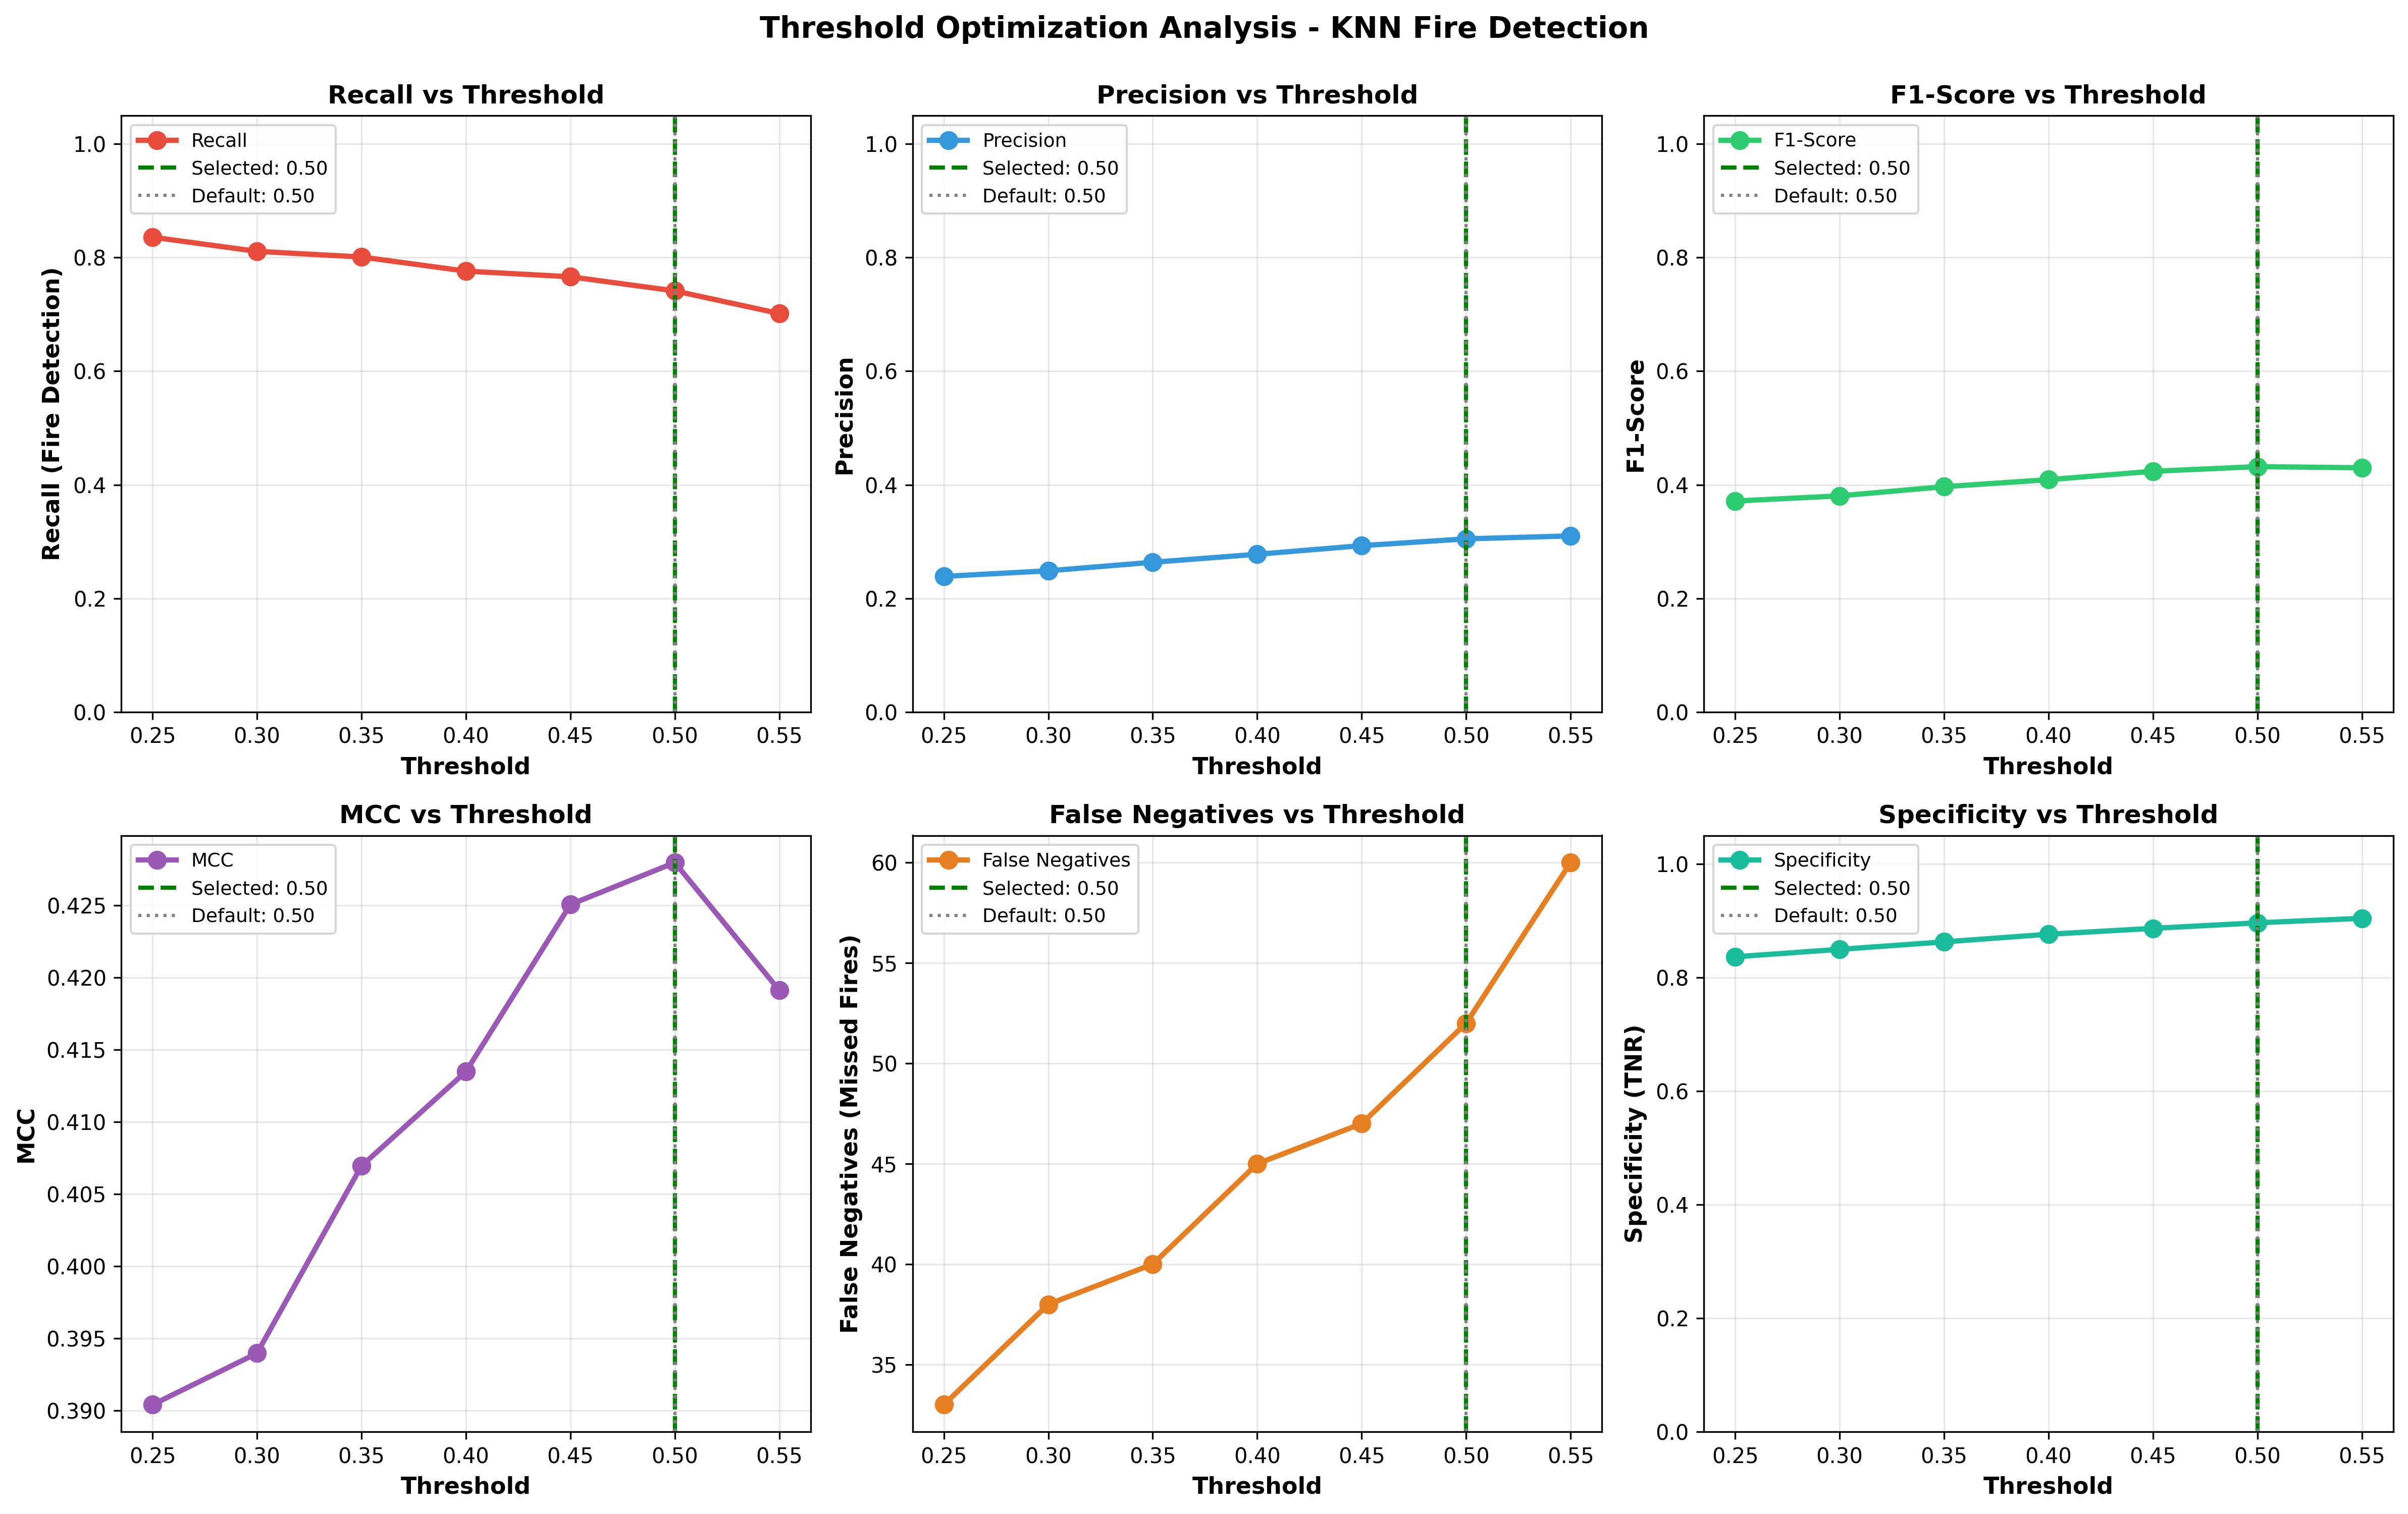
\includegraphics[width=0.5\linewidth]{images/KNN/threshold_optimization_bayesian_KNN_predefined.png}
    \caption{Bayesian threshold optimization results for the predefined KNN model.}
    \label{fig:threshold_optimization_knn_predefined}
\end{figure}




\subsubsection{Predefined vs. Bayesian Optimized KNN Comparison}
Bayesian optimization yields marginal improvements in accuracy, specificity, precision, and F1-score on validation and test sets. Recall decreases slightly, reflecting a trade-off favoring precision. ROC-AUC shows minor degradation, indicating optimization focused on threshold-dependent metrics rather than ranking performance.

\begin{figure}[H]
    \centering
    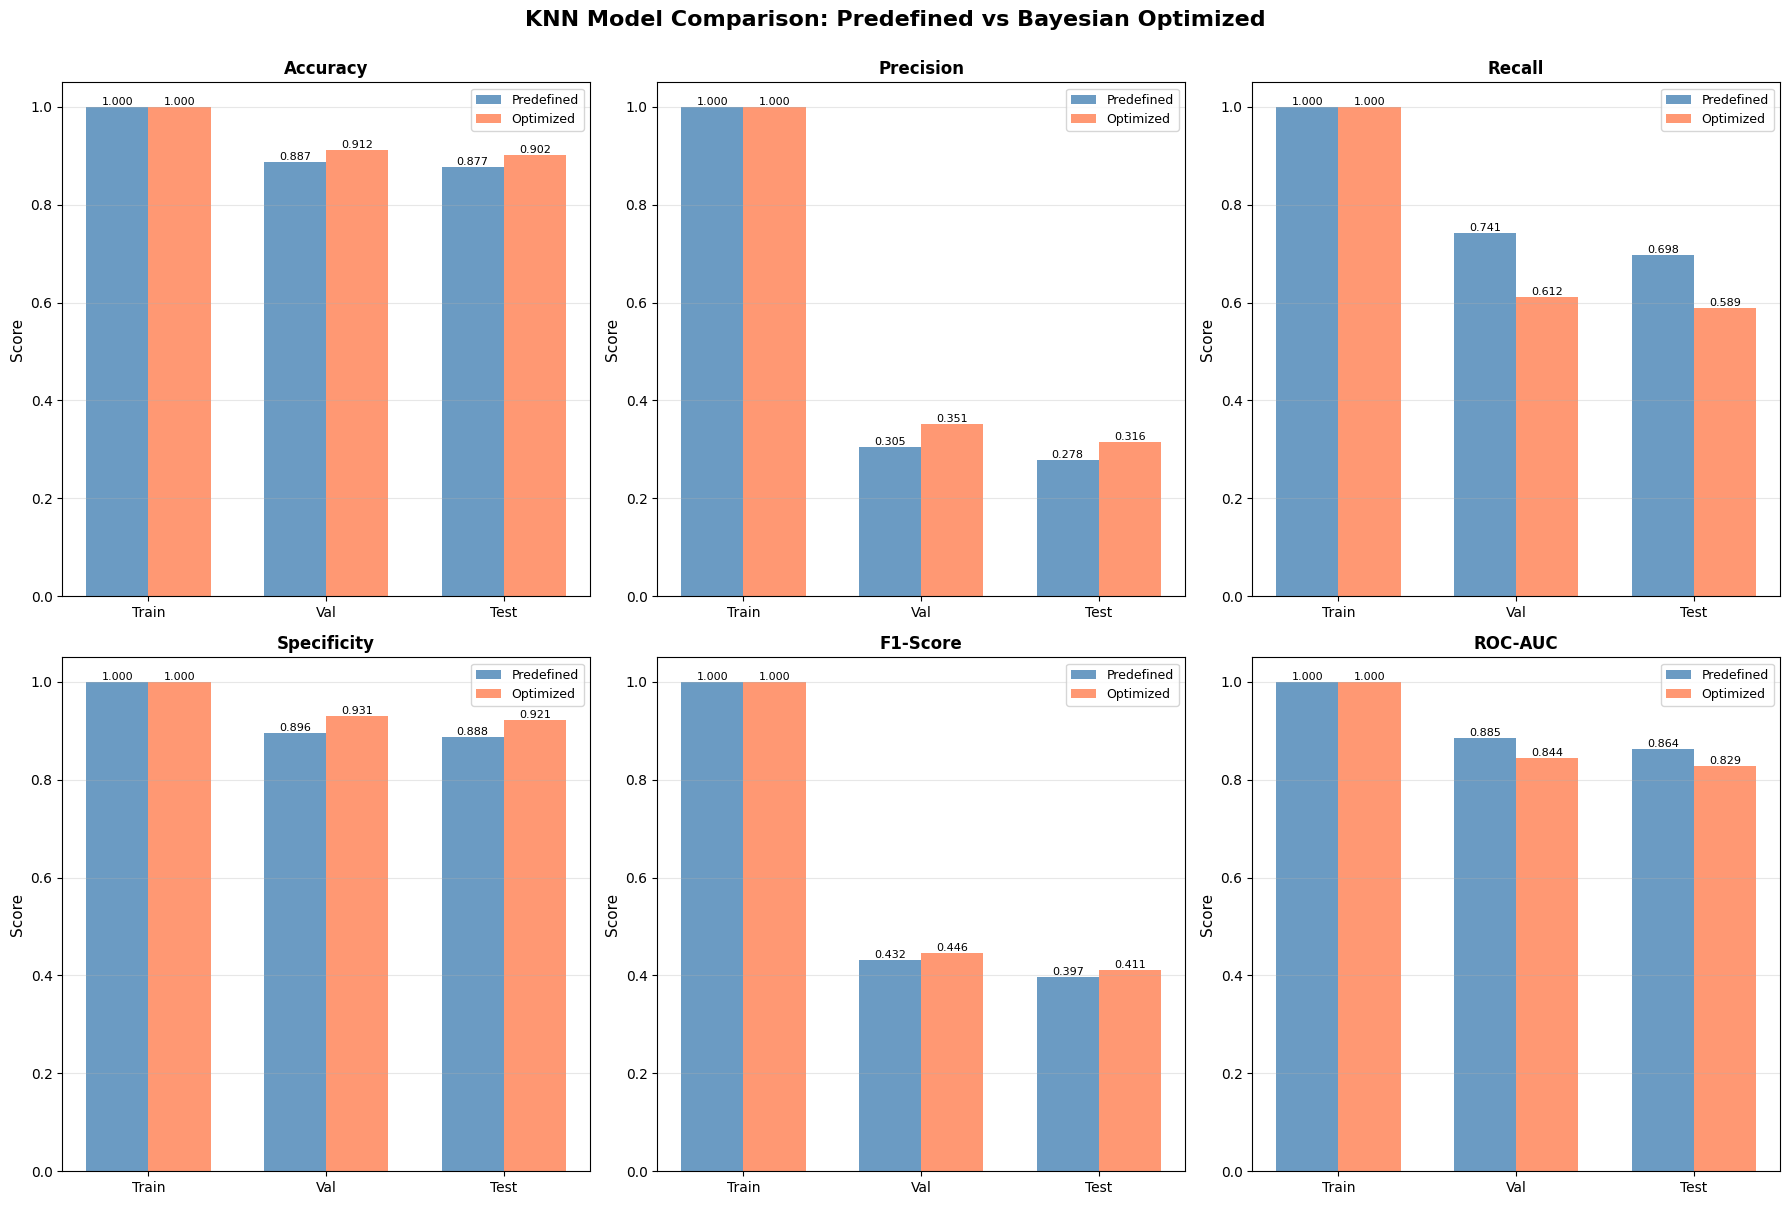
\includegraphics[width=0.5\linewidth]{images/KNN/predefined_vs_optimized_comparison_KNN.png}
    \caption{Comparison of performance metrics between predefined and Bayesian optimized KNN models.}
    \label{fig:metrics_comparison_knn_predefined_vs_bayesian}
\end{figure}

\subsubsection{Bayesian Optimization of KNN}
The Bayesian optimization process converges rapidly, with F1-score stabilizing early, indicating an efficient search. The distribution of F1-scores is tightly concentrated near the optimum (approximately 0.96), demonstrating stable model performance across evaluated configurations.

\begin{figure}[H]
    \centering
    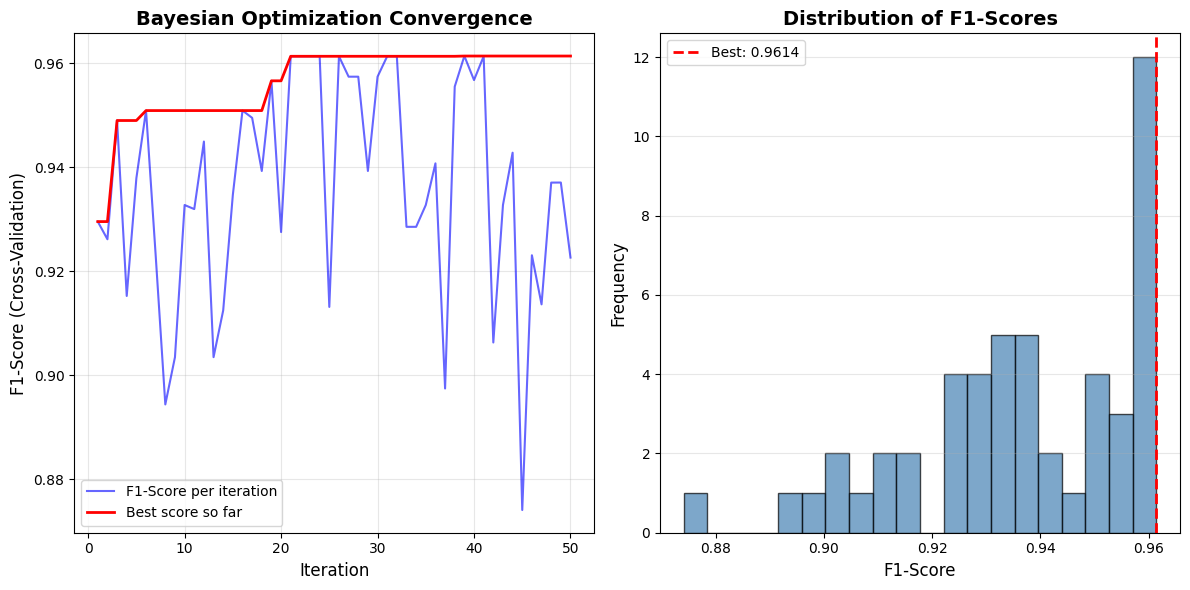
\includegraphics[width=0.5\linewidth]{images/KNN/bayesian_optimization_history_KNN.png}
    \caption{Bayesian optimization process for the predefined KNN model.}
    \label{fig:bayesian_optimization_knn_predefined}
\end{figure}

\subsubsection{Overall Interpretation}
The KNN model exhibits strong ranking ability but is affected by overfitting and class imbalance. Bayesian optimization and threshold tuning improve precision-oriented metrics and stability at the expense of recall, making the final model suitable for applications prioritizing false-positive control.
